\documentclass[aspectratio=169,11pt]{beamer}
\usepackage[T1]{fontenc}
\usepackage{lmodern}
\usepackage{amsmath,amssymb,booktabs}
\usepackage{pgfplots}
\pgfplotsset{compat=1.18}
% Self-contained modern theme: flat typography, generous margins, restrained color.
\usetheme{default}
\definecolor{Ink}{HTML}{142D40}
\definecolor{Teal}{HTML}{008B8B}
\definecolor{Gold}{HTML}{D88B31}
\definecolor{Muted}{HTML}{5B6D7B}
\definecolor{Paper}{HTML}{FAFBFC}
\setbeamercolor{normal text}{fg=Ink,bg=Paper}
\setbeamercolor{structure}{fg=Teal}
\setbeamercolor{frametitle}{fg=Ink}
\setbeamercolor{title}{fg=Ink}
\setbeamercolor{itemize item}{fg=Teal}
\setbeamerfont{title}{size=\Huge,series=\bfseries}
\setbeamerfont{frametitle}{size=\Large,series=\bfseries}
\setbeamersize{text margin left=9mm,text margin right=9mm}
\setbeamertemplate{navigation symbols}{}
\setbeamertemplate{frametitle}{\vspace{5mm}\insertframetitle\par\vspace{2mm}}
\setbeamertemplate{footline}{\hfill\textcolor{Muted}{\scriptsize\insertframenumber\,/\,\inserttotalframenumber}\hspace{9mm}\vspace{4mm}}
\setbeamertemplate{itemize item}{\small\textbullet}
\setlength{\parskip}{5pt}
\newcommand{\sbiaccent}[1]{\textcolor{Teal}{\textbf{#1}}}
\newcommand{\captiontext}[1]{{\scriptsize\color{Muted}#1\par}}
\pgfplotsset{modelplot/.style={width=\linewidth,height=4.5cm,
 axis lines=left,axis line style={Muted},tick label style={font=\scriptsize,color=Muted},
 label style={font=\small},xlabel={$x$},ylabel={$u$},xmin=0,xmax=1,
 grid=major,grid style={gray!12},legend style={font=\scriptsize,draw=none,fill=none,
 at={(0.5,-0.26)},anchor=north,legend columns=3},
 every axis plot/.append style={very thick,no marks},cycle list={{Teal},{Ink,dashed},{Gold,dashdotted}}}}
\title{Small models for\\simulation-based inference}
\subtitle{Four PDE benchmarks in Julia}
\date{October 2026}
\begin{document}

\begin{frame}[plain]
\vspace{10mm}
{\small\color{Teal}\textbf{SBIExamples.jl}}\par\vspace{7mm}
{\usebeamerfont{title}\inserttitle\par}
\vspace{5mm}
{\Large\color{Muted}\insertsubtitle\par}
\vfill
{\small Burgers\quad /\quad Graph transport\quad /\quad Elliptic equations}\par
\vspace{4mm}{\scriptsize\color{Muted}\insertdate}
\end{frame}

\begin{frame}{A common inverse-problem setup}
\[
\underbrace{\theta\sim p(\theta)}_{\text{unknown parameters}}
\quad\longrightarrow\quad
\underbrace{u_h(\theta)}_{\text{numerical PDE solution}}
\quad\longrightarrow\quad
\underbrace{y=H u_h(\theta)+\eta}_{\text{sensor observations}}
\]
\vspace{2mm}
\[\eta\sim\mathcal N(0,\sigma^2 I),\qquad p(\theta\mid y)\propto p(y\mid\theta)p(\theta).\]
\vspace{3mm}
\begin{columns}[T,onlytextwidth]
\column{.46\textwidth}
\sbiaccent{Small by construction}\par
One or two unknowns.\par
32 cells or interior nodes per edge.\par
Eight point sensors per edge.
\column{.48\textwidth}
\sbiaccent{Controlled comparisons}\par
Independent uniform parameter priors.\par
Known noise scale: $\sigma=0.01$ by default.\par
Synthetic data at a known parameter value.
\end{columns}
\end{frame}

\begin{frame}{Four complementary benchmarks}
\renewcommand{\arraystretch}{1.6}
\begin{tabular}{@{}p{3.2cm}p{3.1cm}p{6.0cm}@{}}
\toprule
\textbf{Model} & \textbf{Unknowns} & \textbf{What it probes}\\
\midrule
Viscous Burgers & $\nu,\ A$ & Nonlinear transport and diffusion\\
Graph transport & $c,\ s$ & Travel speed and conservative junction splitting\\
Linear elliptic & $k$ & A reference with an analytic solution\\
Nonlinear elliptic & $\lambda$ & Nonlinear response and iterative forward solves\\
\bottomrule
\end{tabular}
\vspace{5mm}
\sbiaccent{Shared interface:}\quad \texttt{example}\; $\rightarrow$\; \texttt{forward}\; $\rightarrow$\; \texttt{simulate}\; $\rightarrow$\; inference
\end{frame}

\begin{frame}{Viscous Burgers: transport and smoothing}
\begin{columns}[T,onlytextwidth]
\column{.44\textwidth}
\vspace{-4mm}
\[u_t+\partial_x\!\left(\frac{u^2}{2}\right)=\nu u_{xx}\]
Periodic $x\in[0,1]$; observe $t=0.2$.\par
$u(x,0)=A\sin(2\pi x)$.\par
\sbiaccent{Infer viscosity and amplitude}\par
$\nu\sim U(0.01,0.08)$\par
$A\sim U(0.6,1.2)$\par
Truth: $(\nu,A)=(0.03,0.9)$.\par
\small Rusanov finite-volume flux and centered diffusion.
\column{.53\textwidth}
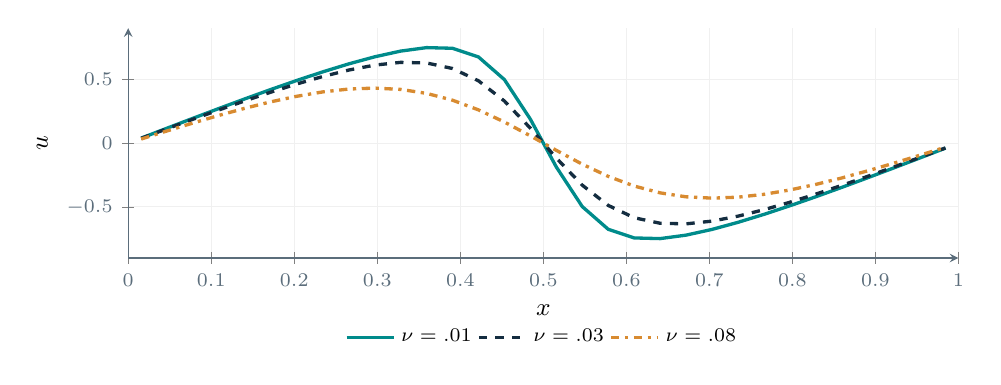
\begin{tikzpicture}\begin{axis}[modelplot,ymin=-0.9,ymax=0.9]
\addplot coordinates {(0.015625,0.039171) (0.046875,0.117336) (0.078125,0.19496) (0.109375,0.271651) (0.140625,0.346958) (0.171875,0.420341) (0.203125,0.491111) (0.234375,0.558342) (0.265625,0.620695) (0.296875,0.676077) (0.328125,0.720864) (0.359375,0.748055) (0.390625,0.742874) (0.421875,0.674897) (0.453125,0.497309) (0.484375,0.187245) (0.515625,-0.187245) (0.546875,-0.497309) (0.578125,-0.674897) (0.609375,-0.742874) (0.640625,-0.748055) (0.671875,-0.720864) (0.703125,-0.676077) (0.734375,-0.620695) (0.765625,-0.558342) (0.796875,-0.491111) (0.828125,-0.420341) (0.859375,-0.346958) (0.890625,-0.271651) (0.921875,-0.19496) (0.953125,-0.117336) (0.984375,-0.039171)};\addlegendentry{$\nu=.01$}
\addplot coordinates {(0.015625,0.037709) (0.046875,0.112873) (0.078125,0.18726) (0.109375,0.260291) (0.140625,0.331283) (0.171875,0.399382) (0.203125,0.463451) (0.234375,0.521889) (0.265625,0.572328) (0.296875,0.611124) (0.328125,0.632563) (0.359375,0.627838) (0.390625,0.584448) (0.421875,0.487999) (0.453125,0.329433) (0.484375,0.117078) (0.515625,-0.117078) (0.546875,-0.329433) (0.578125,-0.487999) (0.609375,-0.584448) (0.640625,-0.627838) (0.671875,-0.632563) (0.703125,-0.611124) (0.734375,-0.572328) (0.765625,-0.521889) (0.796875,-0.463451) (0.828125,-0.399382) (0.859375,-0.331283) (0.890625,-0.260291) (0.921875,-0.18726) (0.953125,-0.112873) (0.984375,-0.037709)};\addlegendentry{$\nu=.03$}
\addplot coordinates {(0.015625,0.032045) (0.046875,0.095656) (0.078125,0.157794) (0.109375,0.217377) (0.140625,0.273155) (0.171875,0.323647) (0.203125,0.367057) (0.234375,0.40121) (0.265625,0.423523) (0.296875,0.431051) (0.328125,0.4207) (0.359375,0.389665) (0.390625,0.336161) (0.421875,0.260341) (0.453125,0.165148) (0.484375,0.056636) (0.515625,-0.056636) (0.546875,-0.165148) (0.578125,-0.260341) (0.609375,-0.336161) (0.640625,-0.389665) (0.671875,-0.4207) (0.703125,-0.431051) (0.734375,-0.423523) (0.765625,-0.40121) (0.796875,-0.367057) (0.828125,-0.323647) (0.859375,-0.273155) (0.890625,-0.217377) (0.921875,-0.157794) (0.953125,-0.095656) (0.984375,-0.032045)};\addlegendentry{$\nu=.08$}
\end{axis}\end{tikzpicture}
\vspace{4mm}\captiontext{Computed profiles at $t=0.2$, $A=0.9$, $n=32$.}
\end{columns}
\end{frame}

\begin{frame}{A hyperbolic conservation law on a graph}
\[\partial_t u_e+\partial_x(cu_e)=0,\qquad e=0,1,2,\quad x\in[0,1].\]
\vspace{1mm}
\begin{columns}[T,onlytextwidth]
\column{.48\textwidth}
\sbiaccent{One parent, two daughter edges}\par
\[\begin{aligned}
q_0&=c\,u_0(1,t),\\
q_1&=c\,u_1(0,t)=s\,q_0,\\
q_2&=c\,u_2(0,t)=(1-s)q_0.
\end{aligned}\]
\[\boxed{q_0=q_1+q_2}\]
\small Zero external inflow; free daughter outflow.
\column{.47\textwidth}
\sbiaccent{Infer speed and the split fraction}\par
$c\sim U(0.6,1.3)$; $s\sim U(0.2,0.8)$.\par
Truth: $(c,s)=(0.9,0.65)$.\par
Observe at $t=0.65$ with 24 sensors.\par
\small Initial parent pulse:
\[u_0(x,0)=\exp\!\left[-\left(\frac{x-0.7}{0.12}\right)^2\right].\]
Daughter edges start at zero.
\end{columns}
\end{frame}

\begin{frame}{Graph transport: the daughter profiles carry the signal}
\begin{columns}[T,onlytextwidth]
\column{.62\textwidth}
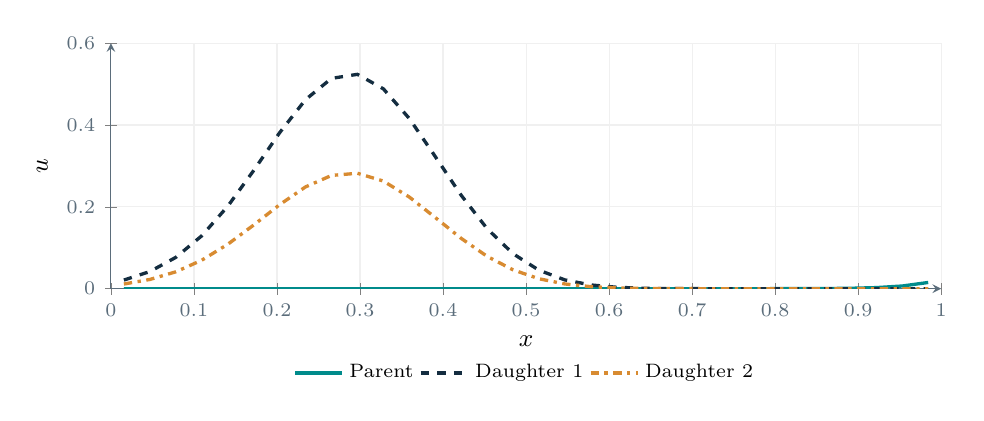
\begin{tikzpicture}\begin{axis}[modelplot,height=4.7cm,ymin=0,ymax=.6]
\addplot coordinates {(0.015625,0.0) (0.046875,0.0) (0.078125,0.0) (0.109375,0.0) (0.140625,0.0) (0.171875,0.0) (0.203125,0.0) (0.234375,0.0) (0.265625,0.0) (0.296875,0.0) (0.328125,0.0) (0.359375,0.0) (0.390625,0.0) (0.421875,0.0) (0.453125,0.0) (0.484375,0.0) (0.515625,0.0) (0.546875,0.0) (0.578125,0.0) (0.609375,0.0) (0.640625,0.0) (0.671875,0.0) (0.703125,1.0e-6) (0.734375,2.0e-6) (0.765625,9.0e-6) (0.796875,3.1e-5) (0.828125,0.000106) (0.859375,0.000333) (0.890625,0.000969) (0.921875,0.002617) (0.953125,0.006543) (0.984375,0.015148)};\addlegendentry{Parent}
\addplot coordinates {(0.015625,0.021095) (0.046875,0.041787) (0.078125,0.076474) (0.109375,0.12918) (0.140625,0.201207) (0.171875,0.288649) (0.203125,0.380943) (0.234375,0.461905) (0.265625,0.513872) (0.296875,0.523765) (0.328125,0.488356) (0.359375,0.415875) (0.390625,0.32292) (0.421875,0.228236) (0.453125,0.146573) (0.484375,0.085362) (0.515625,0.044978) (0.546875,0.021367) (0.578125,0.009089) (0.609375,0.00341) (0.640625,0.001091) (0.671875,0.000278) (0.703125,5.0e-5) (0.734375,4.0e-6) (0.765625,0.0) (0.796875,0.0) (0.828125,0.0) (0.859375,0.0) (0.890625,0.0) (0.921875,0.0) (0.953125,0.0) (0.984375,0.0)};\addlegendentry{Daughter 1}
\addplot coordinates {(0.015625,0.011359) (0.046875,0.022501) (0.078125,0.041178) (0.109375,0.069559) (0.140625,0.108342) (0.171875,0.155427) (0.203125,0.205123) (0.234375,0.248718) (0.265625,0.2767) (0.296875,0.282027) (0.328125,0.262961) (0.359375,0.223933) (0.390625,0.17388) (0.421875,0.122897) (0.453125,0.078924) (0.484375,0.045964) (0.515625,0.024219) (0.546875,0.011505) (0.578125,0.004894) (0.609375,0.001836) (0.640625,0.000588) (0.671875,0.00015) (0.703125,2.7e-5) (0.734375,2.0e-6) (0.765625,0.0) (0.796875,0.0) (0.828125,0.0) (0.859375,0.0) (0.890625,0.0) (0.921875,0.0) (0.953125,0.0) (0.984375,0.0)};\addlegendentry{Daughter 2}
\end{axis}\end{tikzpicture}
\vspace{4mm}\captiontext{Local edge coordinates; $t=0.65$, $c=0.9$, $s=0.65$, $n=32$.}
\column{.34\textwidth}
\sbiaccent{Speed $c$}\par
Controls pulse travel along the network.\par\vspace{3mm}
\sbiaccent{Split $s$}\par
Controls the relative daughter amplitudes.\par\vspace{3mm}
\small Upwind finite volumes preserve the junction flux balance. Mass can leave through the outlets.
\end{columns}
\end{frame}

\begin{frame}{Linear elliptic: an analytic reference}
\begin{columns}[T,onlytextwidth]
\column{.44\textwidth}
\vspace{-4mm}
\[-k u''=1,\qquad x\in(0,1),\]
\[u(0)=u(1)=0.\]
\sbiaccent{Infer conductivity}\par
$k\sim U(0.5,2.0)$; truth $k=1.2$.\par
\[\boxed{u(x;k)=\frac{x(1-x)}{2k}}\]
\small The analytic solution checks the discretization and supports posterior quadrature. Fixing the source avoids scale confounding.
\column{.53\textwidth}
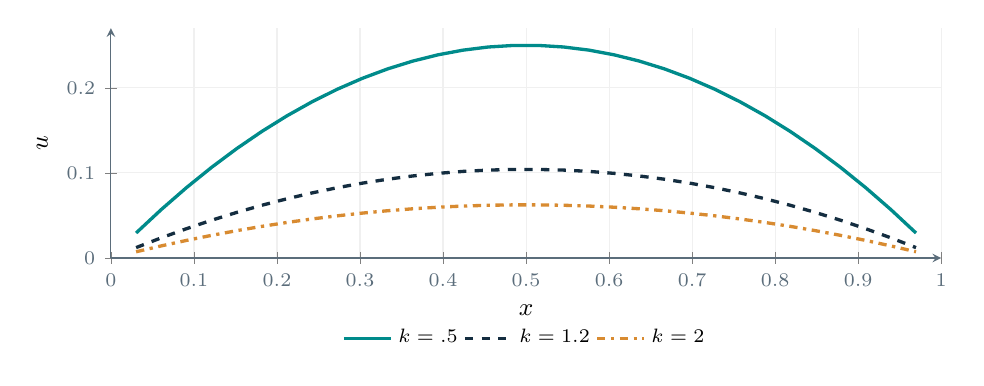
\begin{tikzpicture}\begin{axis}[modelplot,ymin=0,ymax=.27]
\addplot coordinates {(0.030303,0.029385) (0.060606,0.056933) (0.090909,0.082645) (0.121212,0.10652) (0.151515,0.128558) (0.181818,0.14876) (0.212121,0.167126) (0.242424,0.183655) (0.272727,0.198347) (0.30303,0.211203) (0.333333,0.222222) (0.363636,0.231405) (0.393939,0.238751) (0.424242,0.244261) (0.454545,0.247934) (0.484848,0.24977) (0.515152,0.24977) (0.545455,0.247934) (0.575758,0.244261) (0.606061,0.238751) (0.636364,0.231405) (0.666667,0.222222) (0.69697,0.211203) (0.727273,0.198347) (0.757576,0.183655) (0.787879,0.167126) (0.818182,0.14876) (0.848485,0.128558) (0.878788,0.10652) (0.909091,0.082645) (0.939394,0.056933) (0.969697,0.029385)};\addlegendentry{$k=.5$}
\addplot coordinates {(0.030303,0.012244) (0.060606,0.023722) (0.090909,0.034435) (0.121212,0.044383) (0.151515,0.053566) (0.181818,0.061983) (0.212121,0.069636) (0.242424,0.076523) (0.272727,0.082645) (0.30303,0.088001) (0.333333,0.092593) (0.363636,0.096419) (0.393939,0.09948) (0.424242,0.101775) (0.454545,0.103306) (0.484848,0.104071) (0.515152,0.104071) (0.545455,0.103306) (0.575758,0.101775) (0.606061,0.09948) (0.636364,0.096419) (0.666667,0.092593) (0.69697,0.088001) (0.727273,0.082645) (0.757576,0.076523) (0.787879,0.069636) (0.818182,0.061983) (0.848485,0.053566) (0.878788,0.044383) (0.909091,0.034435) (0.939394,0.023722) (0.969697,0.012244)};\addlegendentry{$k=1.2$}
\addplot coordinates {(0.030303,0.007346) (0.060606,0.014233) (0.090909,0.020661) (0.121212,0.02663) (0.151515,0.03214) (0.181818,0.03719) (0.212121,0.041781) (0.242424,0.045914) (0.272727,0.049587) (0.30303,0.052801) (0.333333,0.055556) (0.363636,0.057851) (0.393939,0.059688) (0.424242,0.061065) (0.454545,0.061983) (0.484848,0.062443) (0.515152,0.062443) (0.545455,0.061983) (0.575758,0.061065) (0.606061,0.059688) (0.636364,0.057851) (0.666667,0.055556) (0.69697,0.052801) (0.727273,0.049587) (0.757576,0.045914) (0.787879,0.041781) (0.818182,0.03719) (0.848485,0.03214) (0.878788,0.02663) (0.909091,0.020661) (0.939394,0.014233) (0.969697,0.007346)};\addlegendentry{$k=2$}
\end{axis}\end{tikzpicture}
\vspace{4mm}\captiontext{Centered differences at 32 interior nodes; zero endpoint values.}
\end{columns}
\end{frame}

\begin{frame}{Nonlinear elliptic: reaction changes the response}
\begin{columns}[T,onlytextwidth]
\column{.44\textwidth}
\vspace{-4mm}
\[-u''+\lambda u^3=10,\qquad x\in(0,1),\]
\[u(0)=u(1)=0.\]
\sbiaccent{Infer reaction strength}\par
$\lambda\sim U(0.5,8.0)$; truth $\lambda=4$.\par
\small Centered differences give a nonlinear algebraic system. Damped Newton iterations solve it to a residual tolerance of $10^{-9}$.\par
Larger $\lambda$ suppresses the interior solution.
\column{.53\textwidth}
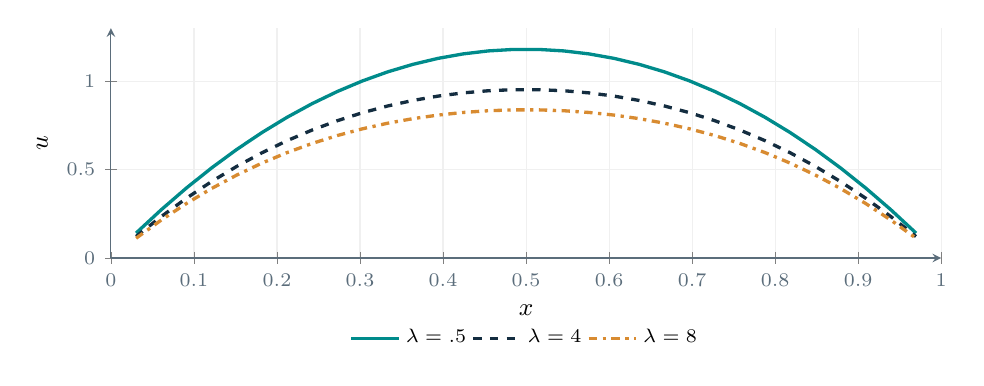
\begin{tikzpicture}\begin{axis}[modelplot,ymin=0,ymax=1.3]
\addplot coordinates {(0.030303,0.141169) (0.060606,0.273156) (0.090909,0.395969) (0.121212,0.509629) (0.151515,0.614167) (0.181818,0.709628) (0.212121,0.79607) (0.242424,0.873562) (0.272727,0.942176) (0.30303,1.001992) (0.333333,1.053088) (0.363636,1.095536) (0.393939,1.129406) (0.424242,1.154754) (0.454545,1.171627) (0.484848,1.180055) (0.515152,1.180055) (0.545455,1.171627) (0.575758,1.154754) (0.606061,1.129406) (0.636364,1.095536) (0.666667,1.053088) (0.69697,1.001992) (0.727273,0.942176) (0.757576,0.873562) (0.787879,0.79607) (0.818182,0.709628) (0.848485,0.614167) (0.878788,0.509629) (0.909091,0.395969) (0.939394,0.273156) (0.969697,0.141169)};\addlegendentry{$\lambda=.5$}
\addplot coordinates {(0.030303,0.12187) (0.060606,0.234564) (0.090909,0.338122) (0.121212,0.43264) (0.151515,0.518272) (0.181818,0.595233) (0.212121,0.663786) (0.242424,0.724231) (0.272727,0.776888) (0.30303,0.822084) (0.333333,0.860139) (0.363636,0.891348) (0.393939,0.915976) (0.424242,0.934244) (0.454545,0.946324) (0.484848,0.952334) (0.515152,0.952334) (0.545455,0.946324) (0.575758,0.934244) (0.606061,0.915976) (0.636364,0.891348) (0.666667,0.860139) (0.69697,0.822084) (0.727273,0.776888) (0.757576,0.724231) (0.787879,0.663786) (0.818182,0.595233) (0.848485,0.518272) (0.878788,0.43264) (0.909091,0.338122) (0.939394,0.234564) (0.969697,0.12187)};\addlegendentry{$\lambda=4$}
\addplot coordinates {(0.030303,0.111989) (0.060606,0.214805) (0.090909,0.308511) (0.121212,0.393251) (0.151515,0.469254) (0.181818,0.536834) (0.212121,0.596367) (0.242424,0.648276) (0.272727,0.693004) (0.30303,0.730994) (0.333333,0.76267) (0.363636,0.788423) (0.393939,0.808593) (0.424242,0.823464) (0.454545,0.833255) (0.484848,0.838113) (0.515152,0.838113) (0.545455,0.833255) (0.575758,0.823464) (0.606061,0.808593) (0.636364,0.788423) (0.666667,0.76267) (0.69697,0.730994) (0.727273,0.693004) (0.757576,0.648276) (0.787879,0.596367) (0.818182,0.536834) (0.848485,0.469254) (0.878788,0.393251) (0.909091,0.308511) (0.939394,0.214805) (0.969697,0.111989)};\addlegendentry{$\lambda=8$}
\end{axis}\end{tikzpicture}
\vspace{4mm}\captiontext{Computed steady states on 32 interior nodes; zero endpoint values.}
\end{columns}
\end{frame}

\begin{frame}{Two inference workflows on the same models}
\begin{columns}[T,onlytextwidth]
\column{.47\textwidth}
\sbiaccent{GpABC.jl: rejection ABC}\par
Draw $\theta$ from the prior; simulate noisy $\widetilde y$. Accept when
\[d(\widetilde y,y)=\frac{\|\widetilde y-y\|_2}{\sigma\sqrt m}\leq\epsilon.\]
Default $\epsilon=2$; equal-weight accepted samples.\par
\small Finite tolerance gives an approximate posterior. Smaller tolerances cost more simulations.
\column{.47\textwidth}
\sbiaccent{SimulationBasedInference.jl: EnIS}\par
Draw a prior ensemble; evaluate noiseless predictions $g(\theta)=H u_h(\theta)$.
\[w_i\propto\exp\!\left[-\frac{\|g(\theta_i)-y\|_2^2}{2\sigma^2}\right].\]
Normalize weights; compute weighted posterior statistics.\par
\small Uses the known Gaussian likelihood as a reference. Check weight degeneracy via effective sample size.
\end{columns}
\vspace{3mm}\captiontext{Here $m$ is the number of sensors. The two methods need not produce identical posteriors.}
\end{frame}

\begin{frame}{A controlled benchmark programme}
\begin{columns}[T,onlytextwidth]
\column{.46\textwidth}
\sbiaccent{Implemented and checked}\par
Four forward models with shared sensors and priors.\par
ABC inference and importance-sampling tests.\par
Analytic elliptic and nonlinear residual checks.\par
Elliptic posterior moments checked against quadrature.
\column{.48\textwidth}
\sbiaccent{Next experiments}\par
Vary sensor placement and measurement noise.\par
Refine the mesh before interpreting physical uncertainty.\par
Compare posterior accuracy at matched simulation budgets.\par
Repeat over synthetic datasets to assess coverage.
\end{columns}
\vspace{4mm}
\captiontext{Current synthetic data and inference use the same mesh. These are small educational benchmarks; mesh convergence and repeated-data calibration remain separate studies.}
\end{frame}

\begin{frame}[fragile]{Code and references}
\sbiaccent{Run the four examples from the repository root}
\begin{verbatim}
julia --project=SBIExamples SBIExamples/examples/run_all.jl
\end{verbatim}
\vspace{3mm}
\sbiaccent{Model definitions and test instructions}\par
\texttt{SBIExamples/src/models.jl}\par
\texttt{SBIExamples/README.md}\par
\vspace{3mm}
\sbiaccent{Inference frameworks}\par
\href{https://github.com/tanhevg/GpABC.jl}{GpABC.jl}\quad\textcolor{Muted}{Rejection approximate Bayesian computation}\par
\href{https://github.com/bgroenks96/SimulationBasedInference.jl}{SimulationBasedInference.jl}\quad\textcolor{Muted}{Ensemble importance sampling}\par
\vspace{3mm}
\captiontext{All plotted curves were computed from the package's forward models at $n=32$. Separate test environments resolve the frameworks' incompatible StatsBase requirements.}
\end{frame}
\end{document}
